\chapter{KMALL stage} \label{ch:kmall_preproc}
Recent advances in sonar technology and computing power have led to an improvement in ocean monitoring. For instance, Multibeam Echosounders (MBES) are now capable of collecting data from the water column, besides some usual metrics such as seafloor reflectivity. This new information allows geoscientists to identify sunken structures, schools of fish, gas seeps, etc.

\begin{figure}[h!]
	\begin{center}
		  \begin{tabular}{ @{} c @{} }
			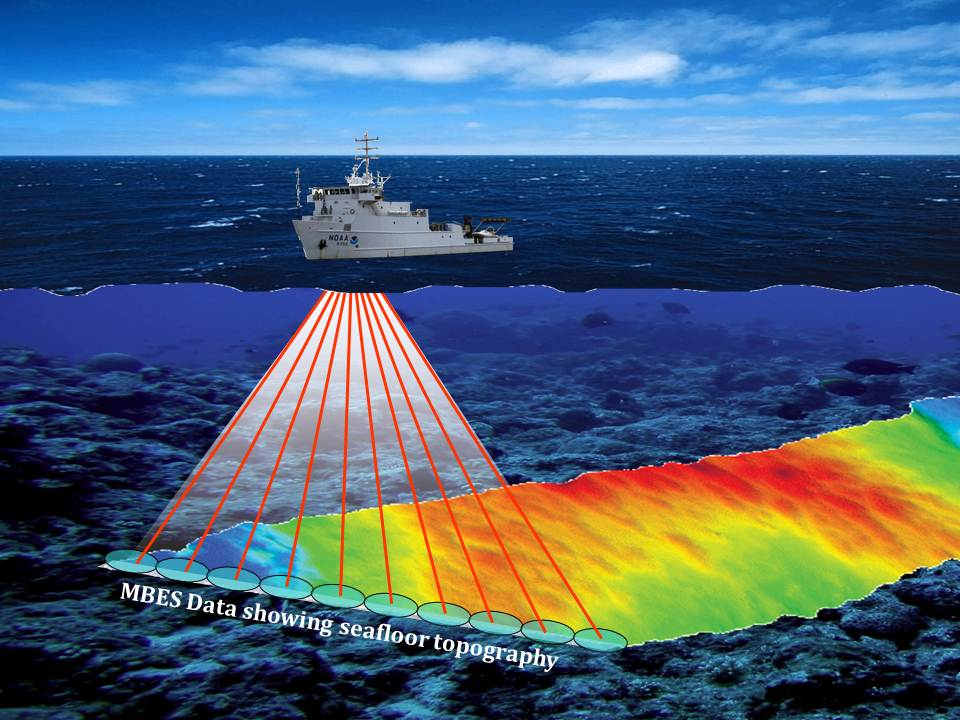
\includegraphics[scale=0.45]{images/mbes_ship.jpg}\\
			\imagesource{NOAA Photo Library, CC BY 2.0, via Wikimedia Commons.}
		\end{tabular}
	\end{center}
	\vspace*{-0.7em}
	\caption{Conception of multibeam sonar on NOAA Ship NANCY FOSTER.}
	\label{fig:mbes_ship}
\end{figure}

We clearly see that water column sensing has a big interest. However, their storage requirements are quite demanding (in the order of some GB/h). Hence, although it is possible to continuously record water column data, in practice it is only used in some specific explorations such as gas-seeps zones. In this scenario, efficient compression algorithms will be essential.

At the present moment, one of the biggest echosounder manufacturers is Kongsberg Maritime, a company with more than 7000 employees over 25 countries. In this chapter we will focus on the development of a preprocessing stage specially designed for the KMALL files from Kongsberg \parencite{KMALL}. First, a general overview of the data structures will be given. Then, with this format in mind, a design criterion will be proposed and implemented. Finally, we will analyze its performance and compare it with other compression algorithms.

\section{The KMALL data format} \label{sec:kmall_format}
In this section we describe the KMALL data structure and why there is a need to develop new compression algorithms for this format, but first, some concepts related to echosounders must be defined:
\begin{itemize}
	\item \textbf{Ping:} A ping is defined as a number of pulses transmitted at approximately the same time.
	\item \textbf{Beam:} Each ping is formed by some pulses in different angles, which we call beams.
\end{itemize}

Notice that the number of beams per ping depends on each sonar model, and the numbers of samples per beam depends on the angle and on the depth. This dependence can be seen in Figure \ref{fig:wc_amplitude}.

The \texttt{.kmall} files use a new format from Kongsberg which is just being implemented in new echosounder models. It is the successor of the Kongsberg \texttt{.all} format. Analyzing the latter is out of the scope of this project, yet we can state some of the improvements that KMALL brings.

On the first hand, KMALL is a generic format with high resolution data and with a datagram structure designed to avoid breaking existing decoders when updating the data structure.

On the other hand, \texttt{.all} format used to have a datagram size constraint of 64 kB due to the maximum size of \acrshort{udp} packets, but \texttt{.kmall} files are designed to be stored "as is" and then fragmented if needed. Its main advantage is that pings are not splitted between datagrams.

The size of a \texttt{.kmall} file is not fixed. Actually, the echosounder operator decides when the file being recorded at that moment should end. In our dataset, kindly provided by Kongsberg Maritime, most of the files are between 100 and 400 MB. Inside these files there are several datagrams, which will be described later.

The mixture of data types in the same file makes it difficult for standard compressors like \textit{Zip} to identify data statistics. Therefore, they do not perform as good as one could expect. In order to improve the compression ratio, we are interested in knowing how are those datagrams placed inside the file and how to identify them. From Kongsberg KMALL documentation, we know that all datagrams start with a generic header that contains the datagram size in bytes and a 4-character identifier. In the current version (410224 Revision H), there are the datagram types listed in tables \ref{tab:first_kmall_table} to \ref{tab:last_kmall_table}.

\begin{table}[H]
\normalsize
\centering
\begin{tabular}{|p{2cm}|p{3.5cm}|p{7.22cm}|}
		\hline
		\rowcolor[HTML]{d6cefc} 
		\multicolumn{1}{|c|}{\cellcolor[HTML]{d6cefc}Type code} & \multicolumn{1}{c|}{\cellcolor[HTML]{d6cefc}Struct name} & \multicolumn{1}{c|}{\cellcolor[HTML]{d6cefc}Description} \\ \hline
		\#CPO                                                   & EMdgmCPO\_def                                            & Compatibility (C) data for position (PO).                \\ \hline
		\#CHE                                                   & EMdgmCHE\_def                                            & Compatibility (C) data for heave (HE).                   \\ \hline
\end{tabular}
\caption{Compatibility datagrams of the KMALL format.}
\label{tab:first_kmall_table}
\end{table}

\begin{table}[h!]
\normalsize
\centering
\begin{tabular}{|p{2cm}|p{3.5cm}|p{7.22cm}|}
	\hline
	\rowcolor[HTML]{d6cefc} 
	\multicolumn{1}{|c|}{\cellcolor[HTML]{d6cefc}Type code} & \multicolumn{1}{c|}{\cellcolor[HTML]{d6cefc}Struct name} & \multicolumn{1}{c|}{\cellcolor[HTML]{d6cefc}Description} \\ \hline
	\#IIP                                                   & EMdgmIIP\_def                                            & Installation and sensor parameters.                      \\ \hline
	\#IOP                                                   & EMdgmIOP\_def                                            & Runtime operator parameters.                             \\ \hline
	\#IBE                                                   & EMdgmIB\_def                                             & Built in test (BIST) error report.                       \\ \hline
	\#IBR                                                   & EMdgmIB\_def                                             & Built in test (BIST) reply.                              \\ \hline
	\#IBS                                                   & EMdgmIB\_def                                             & Built in test (BIST) short reply.                        \\ \hline
\end{tabular}
\caption{Installation and runtime datagrams of the KMALL format.}
\end{table}

\begin{table}[h!]
\normalsize
\centering
\begin{tabular}{|p{2cm}|p{3.5cm}|p{7.22cm}|}
	\hline
	\rowcolor[HTML]{d6cefc} 
	\multicolumn{1}{|c|}{\cellcolor[HTML]{d6cefc}Type code} & \multicolumn{1}{c|}{\cellcolor[HTML]{d6cefc}Struct name} & \multicolumn{1}{c|}{\cellcolor[HTML]{d6cefc}Description}                                              \\ \hline
	\#SPO                                                   & EMdgmSPO\_def                                            & Sensor (S) data for position (PO).                                                                    \\ \hline
	\#SKM                                                   & EMdgmSKM\_def                                            & Sensor (S) KM binary sensor format.                                                                   \\ \hline
	\#SVP                                                   & EMdgmSVP\_def                                            & \begin{tabular}[c]{@{}l@{}}Sensor (S) data from sound velocity (V)\\ profile (P) or CTD.\end{tabular} \\ \hline
	\#SVT                                                   & EMdgmSVT\_def                                            & \begin{tabular}[c]{@{}l@{}}Sensor (S) data for sound velocity (V)\\ at transducer (T).\end{tabular}   \\ \hline
	\#SCL                                                   & EMdgmSCL\_def                                            & Sensor (S) data from clock (CL).                                                                      \\ \hline
	\#SDE                                                   & EMdgmSDE\_def                                            & Sensor (S) data from depth (DE) sensor.                                                               \\ \hline
	\#SHI                                                   & EMdgmSHI\_def                                            & Sensor (S) data for height (HI).                                                                      \\ \hline
\end{tabular}
\caption{External sensor output datagrams of the KMALL format.}
\end{table}

\begin{table}[h!]
\normalsize
\centering
\begin{tabular}{|p{2cm}|p{3.5cm}|p{7.22cm}|}
	\hline
	\rowcolor[HTML]{d6cefc}
	\multicolumn{1}{|c|}{\cellcolor[HTML]{d6cefc}Type code} & \multicolumn{1}{c|}{\cellcolor[HTML]{d6cefc}Struct name} & \multicolumn{1}{c|}{\cellcolor[HTML]{d6cefc}Description} \\ \hline
	\#FCF                                                   & EMdgmFCF\_def                                            & \begin{tabular}[c]{@{}l@{}}Backscatter calibration (C) file (F) \\ datagram.\end{tabular}   \\ \hline
\end{tabular}
\caption{File datagrams of the KMALL format.}
\end{table}

\begin{table}[h!]
\normalsize
\centering
\begin{tabular}{|p{2cm}|p{3.5cm}|p{7.22cm}|}
		\hline
		\rowcolor[HTML]{d6cefc} 
		\multicolumn{1}{|c|}{\cellcolor[HTML]{d6cefc}Type code} & \multicolumn{1}{c|}{\cellcolor[HTML]{d6cefc}Struct name} & \multicolumn{1}{c|}{\cellcolor[HTML]{d6cefc}Description}                                      \\ \hline
		\#MRZ                                                   & EMdgmMRZ\_def                                            & \begin{tabular}[c]{@{}l@{}}Multibeam (M) raw range (R)\\ and depth (Z) datagram.\end{tabular} \\ \hline
		\#MWC                                                   & EMdgmMWC\_def                                            & \begin{tabular}[c]{@{}l@{}}Multibeam (M) water (W)\\ column (C) datagram.\end{tabular}        \\ \hline
\end{tabular}
\caption{Multibeam datagrams of the KMALL format.}
\label{tab:last_kmall_table}
\end{table}

It is important to notice that a given \texttt{.kmall} file can contain all the above datagrams. However, we may usually find that water column data is logged in a separate file with extension \texttt{.kmwcd}. In other words, MWC datagrams will be stored in \texttt{.kmwcd} files instead of \texttt{.kmall} files, but the decoding process is the same for both extensions as the data format is exactly the same.

As we will see in the next section, our main interest in this chapter will lie in MWC datagrams. Therefore, before continuing, an appropriate description of them shall be given.

\pagebreak
MWC datagrams are structured as follows:

\begin{figure}[h!]
	\begin{center}
		\scalebox{.565}{% Graphic for TeX using PGF
% Title: /home/aniol/Documents/Uni/Telecos/TFG/mwc_datagram.dia
% Creator: Dia v0.97+git
% CreationDate: Fri Feb 12 18:10:30 2021
% For: aniol
% \usepackage{tikz}
% The following commands are not supported in PSTricks at present
% We define them conditionally, so when they are implemented,
% this pgf file will use them.
\ifx\du\undefined
  \newlength{\du}
\fi
\setlength{\du}{15\unitlength}
\begin{tikzpicture}[even odd rule]
\pgftransformxscale{1.000000}
\pgftransformyscale{-1.000000}
\definecolor{dialinecolor}{rgb}{0.000000, 0.000000, 0.000000}
\pgfsetstrokecolor{dialinecolor}
\pgfsetstrokeopacity{1.000000}
\definecolor{diafillcolor}{rgb}{1.000000, 1.000000, 1.000000}
\pgfsetfillcolor{diafillcolor}
\pgfsetfillopacity{1.000000}
\pgfsetlinewidth{0.100000\du}
\pgfsetdash{}{0pt}
\pgfsetmiterjoin
\pgfsetbuttcap
{\pgfsetcornersarced{\pgfpoint{0.000000\du}{0.000000\du}}\definecolor{diafillcolor}{rgb}{1.000000, 1.000000, 1.000000}
\pgfsetfillcolor{diafillcolor}
\pgfsetfillopacity{1.000000}
\fill (2.100000\du,9.900000\du)--(2.100000\du,15.000000\du)--(52.000000\du,15.000000\du)--(52.000000\du,9.900000\du)--cycle;
}{\pgfsetcornersarced{\pgfpoint{0.000000\du}{0.000000\du}}\definecolor{dialinecolor}{rgb}{0.000000, 0.000000, 0.000000}
\pgfsetstrokecolor{dialinecolor}
\pgfsetstrokeopacity{1.000000}
\draw (2.100000\du,9.900000\du)--(2.100000\du,15.000000\du)--(52.000000\du,15.000000\du)--(52.000000\du,9.900000\du)--cycle;
}\pgfsetlinewidth{0.100000\du}
\pgfsetdash{}{0pt}
\pgfsetbuttcap
{
\definecolor{diafillcolor}{rgb}{0.000000, 0.000000, 0.000000}
\pgfsetfillcolor{diafillcolor}
\pgfsetfillopacity{1.000000}
% was here!!!
\definecolor{dialinecolor}{rgb}{0.000000, 0.000000, 0.000000}
\pgfsetstrokecolor{dialinecolor}
\pgfsetstrokeopacity{1.000000}
\draw (7.058330\du,9.850000\du)--(7.058330\du,15.031300\du);
}
% setfont left to latex
\definecolor{dialinecolor}{rgb}{0.000000, 0.000000, 0.000000}
\pgfsetstrokecolor{dialinecolor}
\pgfsetstrokeopacity{1.000000}
\definecolor{diafillcolor}{rgb}{0.000000, 0.000000, 0.000000}
\pgfsetfillcolor{diafillcolor}
\pgfsetfillopacity{1.000000}
\node[anchor=base,inner sep=0pt, outer sep=0pt,color=dialinecolor] at (4.516770\du,12.193700\du){Header};
% setfont left to latex
\definecolor{dialinecolor}{rgb}{0.000000, 0.000000, 0.000000}
\pgfsetstrokecolor{dialinecolor}
\pgfsetstrokeopacity{1.000000}
\definecolor{diafillcolor}{rgb}{0.000000, 0.000000, 0.000000}
\pgfsetfillcolor{diafillcolor}
\pgfsetfillopacity{1.000000}
\node[anchor=base,inner sep=0pt, outer sep=0pt,color=dialinecolor] at (4.516770\du,12.993700\du){20 \ensuremath{[}B\ensuremath{]}};
\pgfsetlinewidth{0.100000\du}
\pgfsetdash{}{0pt}
\pgfsetbuttcap
{
\definecolor{diafillcolor}{rgb}{0.000000, 0.000000, 0.000000}
\pgfsetfillcolor{diafillcolor}
\pgfsetfillopacity{1.000000}
% was here!!!
\definecolor{dialinecolor}{rgb}{0.000000, 0.000000, 0.000000}
\pgfsetstrokecolor{dialinecolor}
\pgfsetstrokeopacity{1.000000}
\draw (10.606800\du,9.867080\du)--(10.606800\du,15.048300\du);
}
% setfont left to latex
\definecolor{dialinecolor}{rgb}{0.000000, 0.000000, 0.000000}
\pgfsetstrokecolor{dialinecolor}
\pgfsetstrokeopacity{1.000000}
\definecolor{diafillcolor}{rgb}{0.000000, 0.000000, 0.000000}
\pgfsetfillcolor{diafillcolor}
\pgfsetfillopacity{1.000000}
\node[anchor=base,inner sep=0pt, outer sep=0pt,color=dialinecolor] at (8.850100\du,12.193800\du){Partition};
% setfont left to latex
\definecolor{dialinecolor}{rgb}{0.000000, 0.000000, 0.000000}
\pgfsetstrokecolor{dialinecolor}
\pgfsetstrokeopacity{1.000000}
\definecolor{diafillcolor}{rgb}{0.000000, 0.000000, 0.000000}
\pgfsetfillcolor{diafillcolor}
\pgfsetfillopacity{1.000000}
\node[anchor=base,inner sep=0pt, outer sep=0pt,color=dialinecolor] at (8.850100\du,12.993800\du){4 \ensuremath{[}B\ensuremath{]}};
\pgfsetlinewidth{0.100000\du}
\pgfsetdash{}{0pt}
\pgfsetbuttcap
{
\definecolor{diafillcolor}{rgb}{0.000000, 0.000000, 0.000000}
\pgfsetfillcolor{diafillcolor}
\pgfsetfillopacity{1.000000}
% was here!!!
\definecolor{dialinecolor}{rgb}{0.000000, 0.000000, 0.000000}
\pgfsetstrokecolor{dialinecolor}
\pgfsetstrokeopacity{1.000000}
\draw (15.140100\du,9.867080\du)--(15.140100\du,15.048300\du);
}
% setfont left to latex
\definecolor{dialinecolor}{rgb}{0.000000, 0.000000, 0.000000}
\pgfsetstrokecolor{dialinecolor}
\pgfsetstrokeopacity{1.000000}
\definecolor{diafillcolor}{rgb}{0.000000, 0.000000, 0.000000}
\pgfsetfillcolor{diafillcolor}
\pgfsetfillopacity{1.000000}
\node[anchor=base,inner sep=0pt, outer sep=0pt,color=dialinecolor] at (12.883400\du,12.193800\du){CmnPart};
% setfont left to latex
\definecolor{dialinecolor}{rgb}{0.000000, 0.000000, 0.000000}
\pgfsetstrokecolor{dialinecolor}
\pgfsetstrokeopacity{1.000000}
\definecolor{diafillcolor}{rgb}{0.000000, 0.000000, 0.000000}
\pgfsetfillcolor{diafillcolor}
\pgfsetfillopacity{1.000000}
\node[anchor=base,inner sep=0pt, outer sep=0pt,color=dialinecolor] at (12.883400\du,12.993800\du){12 \ensuremath{[}B\ensuremath{]}};
\pgfsetlinewidth{0.100000\du}
\pgfsetdash{}{0pt}
\pgfsetbuttcap
{
\definecolor{diafillcolor}{rgb}{0.000000, 0.000000, 0.000000}
\pgfsetfillcolor{diafillcolor}
\pgfsetfillopacity{1.000000}
% was here!!!
\definecolor{dialinecolor}{rgb}{0.000000, 0.000000, 0.000000}
\pgfsetstrokecolor{dialinecolor}
\pgfsetstrokeopacity{1.000000}
\draw (19.780100\du,9.857080\du)--(19.780100\du,15.038300\du);
}
% setfont left to latex
\definecolor{dialinecolor}{rgb}{0.000000, 0.000000, 0.000000}
\pgfsetstrokecolor{dialinecolor}
\pgfsetstrokeopacity{1.000000}
\definecolor{diafillcolor}{rgb}{0.000000, 0.000000, 0.000000}
\pgfsetfillcolor{diafillcolor}
\pgfsetfillopacity{1.000000}
\node[anchor=base,inner sep=0pt, outer sep=0pt,color=dialinecolor] at (17.483400\du,12.193700\du){TxInfo};
% setfont left to latex
\definecolor{dialinecolor}{rgb}{0.000000, 0.000000, 0.000000}
\pgfsetstrokecolor{dialinecolor}
\pgfsetstrokeopacity{1.000000}
\definecolor{diafillcolor}{rgb}{0.000000, 0.000000, 0.000000}
\pgfsetfillcolor{diafillcolor}
\pgfsetfillopacity{1.000000}
\node[anchor=base,inner sep=0pt, outer sep=0pt,color=dialinecolor] at (17.483400\du,12.993700\du){12 \ensuremath{[}B\ensuremath{]}};
\pgfsetlinewidth{0.100000\du}
\pgfsetdash{}{0pt}
\pgfsetbuttcap
{
\definecolor{diafillcolor}{rgb}{0.000000, 0.000000, 0.000000}
\pgfsetfillcolor{diafillcolor}
\pgfsetfillopacity{1.000000}
% was here!!!
\definecolor{dialinecolor}{rgb}{0.000000, 0.000000, 0.000000}
\pgfsetstrokecolor{dialinecolor}
\pgfsetstrokeopacity{1.000000}
\draw (27.206700\du,9.865000\du)--(27.206700\du,15.046200\du);
}
% setfont left to latex
\definecolor{dialinecolor}{rgb}{0.000000, 0.000000, 0.000000}
\pgfsetstrokecolor{dialinecolor}
\pgfsetstrokeopacity{1.000000}
\definecolor{diafillcolor}{rgb}{0.000000, 0.000000, 0.000000}
\pgfsetfillcolor{diafillcolor}
\pgfsetfillopacity{1.000000}
\node[anchor=base,inner sep=0pt, outer sep=0pt,color=dialinecolor] at (23.516700\du,12.158400\du){SectorData};
% setfont left to latex
\definecolor{dialinecolor}{rgb}{0.000000, 0.000000, 0.000000}
\pgfsetstrokecolor{dialinecolor}
\pgfsetstrokeopacity{1.000000}
\definecolor{diafillcolor}{rgb}{0.000000, 0.000000, 0.000000}
\pgfsetfillcolor{diafillcolor}
\pgfsetfillopacity{1.000000}
\node[anchor=base,inner sep=0pt, outer sep=0pt,color=dialinecolor] at (23.516700\du,12.958400\du){9 x 16 \ensuremath{[}B\ensuremath{]}};
\pgfsetlinewidth{0.100000\du}
\pgfsetdash{}{0pt}
\pgfsetbuttcap
{
\definecolor{diafillcolor}{rgb}{0.000000, 0.000000, 0.000000}
\pgfsetfillcolor{diafillcolor}
\pgfsetfillopacity{1.000000}
% was here!!!
\definecolor{dialinecolor}{rgb}{0.000000, 0.000000, 0.000000}
\pgfsetstrokecolor{dialinecolor}
\pgfsetstrokeopacity{1.000000}
\draw (32.580000\du,9.855000\du)--(32.580000\du,15.036200\du);
}
% setfont left to latex
\definecolor{dialinecolor}{rgb}{0.000000, 0.000000, 0.000000}
\pgfsetstrokecolor{dialinecolor}
\pgfsetstrokeopacity{1.000000}
\definecolor{diafillcolor}{rgb}{0.000000, 0.000000, 0.000000}
\pgfsetfillcolor{diafillcolor}
\pgfsetfillopacity{1.000000}
\node[anchor=base,inner sep=0pt, outer sep=0pt,color=dialinecolor] at (29.950000\du,12.158300\du){RxInfo};
% setfont left to latex
\definecolor{dialinecolor}{rgb}{0.000000, 0.000000, 0.000000}
\pgfsetstrokecolor{dialinecolor}
\pgfsetstrokeopacity{1.000000}
\definecolor{diafillcolor}{rgb}{0.000000, 0.000000, 0.000000}
\pgfsetfillcolor{diafillcolor}
\pgfsetfillopacity{1.000000}
\node[anchor=base,inner sep=0pt, outer sep=0pt,color=dialinecolor] at (29.950000\du,12.958300\du){16 \ensuremath{[}B\ensuremath{]}};
% setfont left to latex
\definecolor{dialinecolor}{rgb}{0.000000, 0.000000, 0.000000}
\pgfsetstrokecolor{dialinecolor}
\pgfsetstrokeopacity{1.000000}
\definecolor{diafillcolor}{rgb}{0.000000, 0.000000, 0.000000}
\pgfsetfillcolor{diafillcolor}
\pgfsetfillopacity{1.000000}
\node[anchor=base,inner sep=0pt, outer sep=0pt,color=dialinecolor] at (42.150000\du,12.125000\du){BeamData};
% setfont left to latex
\definecolor{dialinecolor}{rgb}{0.000000, 0.000000, 0.000000}
\pgfsetstrokecolor{dialinecolor}
\pgfsetstrokeopacity{1.000000}
\definecolor{diafillcolor}{rgb}{0.000000, 0.000000, 0.000000}
\pgfsetfillcolor{diafillcolor}
\pgfsetfillopacity{1.000000}
\node[anchor=base,inner sep=0pt, outer sep=0pt,color=dialinecolor] at (42.150000\du,12.925000\du){$N_B \cdot (16 + N_S \cdot (1 + phaseFlag))$ \ensuremath{[}B\ensuremath{]}};
\end{tikzpicture}
}
	\end{center}
	\caption{MWC datagram as described by Kongsberg (410224 Revision H).}
	\label{fig:mwc_datagram}
\end{figure}
Where:
\begin{description}
	\item $N_B \equiv$ Number of beams in ping. It is stored as a 16-bit integer in \textit{RxInfo}.
	\item $N_S \equiv$ Number of samples in beam. It is stored as a 16-bit integer in \textit{BeamData}.
	\item $phaseFlag \equiv$ Flag that indicates if there is phase information after amplitude samples. It may be 0 (no phase information), 1 (8-bit resolution) or 2 (16-bit resolution). It is stored as an 8-bit integer in \textit{RxInfo}.
\end{description}

In the present work we will only use information contained in \textit{Header} such as the datagram size and the datagram type, in \textit{RxInfo} and in \textit{BeamData}. For further details, the interested reader is referred to \parencite{KMALL}.

\section{Design}
We have already described the KMALL format and we have also justified why this stage is needed. Now it is time to start designing an algorithm to decorrelate the data in these files. We will follow a two-step approach: first we will analyze the KMALL files in our dataset to determine which of the datagrams listed in section \ref{sec:kmall_format} are worth to be compressed. Then, we will propose an algorithm that suits the requirements stated in section \ref{sec:requirements}. There are no specific requirements for this stage.

\subsection{Data analysis} \label{sec:kmall_analysis}
In order to decide what to compress, we have first analyzed some \texttt{.kmall} and \texttt{.kmwcd} files to determine the percentage of occupancy by datagram type. The procedure we have followed is the following:
\begin{enumerate}
	\item Implement the existing C++ KMALL format in Python.
	\item Implement a Python class which acts as top level \acrshort{api} for the KMALL files.
	\item Write a Python script that takes a directory and an extension and returns the percentages of every datagram type.
\end{enumerate}
The result is that for \texttt{.kmall} files, MRZ datagrams are a 92\% of the total size; and for \texttt{.kmwcd}, \acrshort{mwc} datagrams are a 99\%. From this evaluation it is clear that these two data types are our objective; however, they are too different to be preprocessed with the same stage, therefore in this thesis we will ignore MRZ datagrams and we will just focus on \acrshort{mwc} data.

If we look closer at a MWC datagram (see Figure \ref{fig:mwc_datagram}) we see that all the headers size is insignificant compared with the samples volume. Hence, we will only compress the payload, which includes amplitude and phase information.

In conclusion, we will design a stage which will only give some special attention to the information contained in the \textit{BeamData} subdatagram from MWC datagrams.

\subsection{Algorithm design}
In 2019, DAPCOM developed a \acrshort{fapec} stage to compress \acrshort{mwc} data contained in \texttt{.wcd} files \parencite{Portell2019}, the predecessor of \texttt{.kmwcd}. For this reason, the stage we are presenting here is not strictly new, but an adaption of an already existing one.

Our first concern is \acrshort{fapec} data chunking. This feature may be dangerous because splitting a datagram into different chunks is not desirable as it complicates file reading. For this reason, assuming a degradation in performance, we will allow chunks with a true size smaller than the chunk size set by the user. We should remark that even with this constraint, the chunk size will be typically between 1 MB and 2 MB, therefore fulfilling specification \ref{spec:chunk_size}.

The second step is to identify MWC datagrams. To do that, we just need to read the datagram type field in the header. If it is a MWC datagram, a custom algorithm is applied. Otherwise, samples are directly sent to the entropy encoder.

Now it is time to focus on the payload data and how can we decorrelate it. If we represent the amplitude samples as a raw rectangular image (see Figure \ref{fig:wc_amplitude}) we can see that correlation between beams is higher than between samples (i.e. the image is smoother from top to bottom than left to right). Although this is purely qualitative, it matches with the algorithm designed in \parencite{Portell2019}, and it can be proved to be true by applying a simple differential first by rows and then by columns and finally comparing the results. In the picture we can also see that the number of samples per beam is not constant, but it has a parabolic behavior.
\begin{figure}[h!]
	\begin{center}
		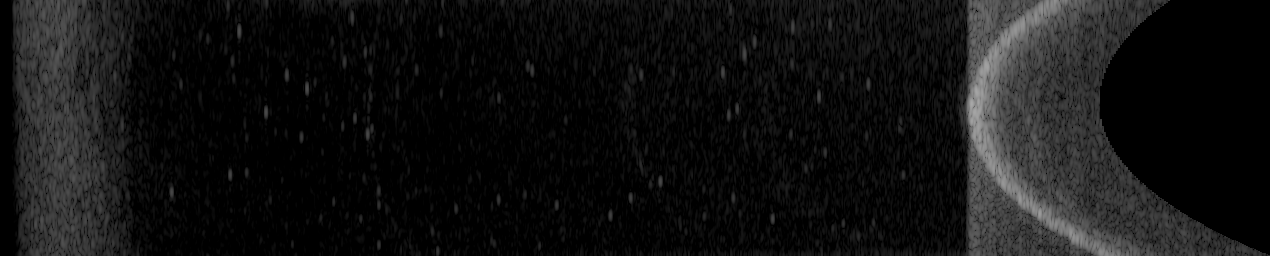
\includegraphics[scale=0.334]{images/water_column_amp.png}
	\end{center}
	\caption{Raw representation of \acrshort{mwc} amplitude from a EM 2040 echosounder.}
	\label{fig:wc_amplitude}
\end{figure}

In the implementation for \texttt{.wcd} files, given a sample $S_{i,j}$ in the position $i$ of the beam $j$, the vertex coordinates $(V_x, V_y)$ and the number of beams $N_B$, prediction errors $E_{i,j}$ in the rectangular region are calculated:
\begin{equation}
E_{i,j} = S_{i,j} - S_{i,j-1}, \qquad 0 \leq i < V_x, \quad 1 \leq j < N_B.
\end{equation}

In other words, the samples from the rectangular region are predicted from the samples in the same position as those from the previous beam.

The remaining samples are predicted following a simple differential between them and a correction coefficient. Formally, given $N_{S_j}$ the number of samples in the beam $j$, then
\begin{equation}
E_{i,j} = S_{i,j} - S_{i-1,j} - C_{i,j}, \qquad Vx \leq i < N_{S_j}, \quad 1 \leq j < N_B
\end{equation}
where $C_{i,j}$ is given by:
\begin{equation}
C_{i,j} = \frac{1}{16}(7E_{i-1,j} + 6E_{i-2,j} + 4E_{i-3,j} + 3E_{i-4,j}).
\end{equation}

As the reader may have noticed, these equations are not defined for $j=0$ (i.e. the first beam). The reason is that the system must be causal, therefore the first beam is predicted from the previous sample in the same beam:
\begin{equation} \label{eq:first_beam}
E_{i,0} = S_{i,0} - S_{i-1,0}, \qquad 1 \leq i < N_{S_0}.
\end{equation}

The algorithm we propose in this thesis is very similar to the one we have just described for \texttt{.wcd} files, but with some improvements. We also follow the approach of predicting samples from the previous beam, but we do not restrict to the square region. Instead, we do that for all the samples which have a sample above. Formally,
\begin{equation}
E_{i,j} = S_{i,j} - S_{i,j-1}, \qquad 0 \leq i < \min(N_{S_{j-1}}, N_{S_j}), \quad 1 \leq j < N_B.
\end{equation}

The remaining samples are predicted with the previous samples. Mathematically,
\begin{equation} \label{eq:samples}
E_{i,j} = S_{i,j} - S_{i-1,j}, \qquad \min(N_{S_{j-1}}, N_{S_j}) \leq i < N_{S_j}, \quad 1 \leq j < N_B.
\end{equation}

The prediction errors for the first beam are also calculated with Equation \ref{eq:first_beam}, with the addition that
\begin{equation}
E_{0,0} = S_{0,0} + 128.
\end{equation}

Now we are interested in observing if this algorithm also work for the phase information present in MWC datagrams. Notice that the former stage for \texttt{.wcd} was not designed to work with phase samples. In Figure \ref{fig:wc_phase} we show the phase corresponding to the amplitudes in Figure \ref{fig:wc_amplitude}. As the reader can see, this information is almost white noise, therefore it is theoretically impossible to compress. Our final decision has been to apply a simple differential between samples (i.e. Equation \ref{eq:samples}).
\begin{figure}[h!]
	\begin{center}
		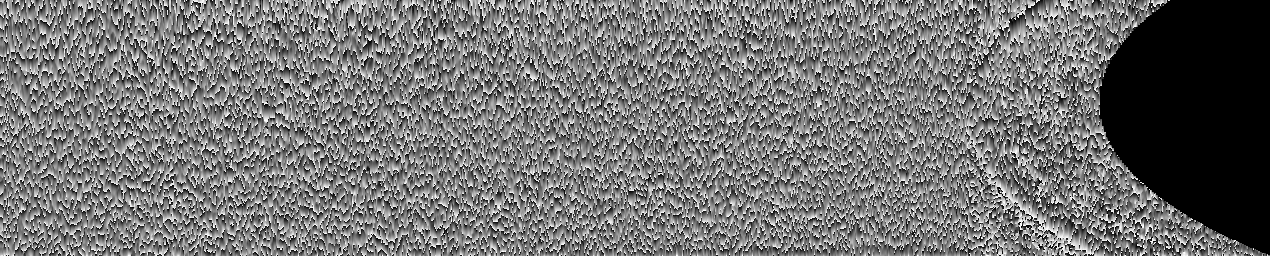
\includegraphics[scale=0.334]{images/water_column_ph.png}
	\end{center}
	\caption{Raw representation of \acrshort{mwc} phase from a EM 2040 echosounder.}
	\label{fig:wc_phase}
\end{figure}

Finally, we should remark that more complex algorithms like nearest-neighbor or a generic linear predictor of order $Q$ have been tested, but they are slower and also have a worse compression ratio.

\pagebreak
In Figure \ref{fig:kmall_flowchart} a flowchart for the KMALL stage is included, where \textit{Settings} are two parameters: amplitude and phase losses levels.

\begin{figure}[h!]
	\begin{center}
		\scalebox{.95}{\begin{tikzpicture}[
        every node/.style={draw,minimum width=3cm,minimum height=1cm},
        every text node part/.style={align=center},
         node distance=2.6cm and 3.8cm, on grid,
        >={Stealth[length=2mm]},
        inici/.style={rounded rectangle,minimum height=1cm,fill=ForestGreen!20},
        parametres/.style={
            trapezium,
            shape border rotate=90,
            trapezium left angle=90, 
            trapezium right angle=80,
            minimum width=1cm,
            fill=yellow!30,
        },
        entrada/.style={tape,minimum width=1.5cm,fill=violet!20},
        rectangle/.style={minimum width=2.2cm,fill=blue!10},
        decisio/.style={diamond,minimum height=1.7cm,aspect=1.6,fill=red!10},
        coordenada/.style={draw=none,minimum width=0},
        bool/.style={draw=none,minimum width=0,minimum height=0},
    ]
    \scriptsize
    % Dibuixo primer els nodes i després les fletxes. Hi ha diverses maneres de fer-ho
    \node[inici,minimum width=4cm] (start) {Start};
    \node[entrada] (input) at (-1.3,2) {Input file};
    \node[parametres] (settings) at (1,2) {Settings};
    \node[decisio,below=of start] (D1) {Read bytes =\\buffer size?};
    \node[inici, right=of D1] (end) {End};
    \node[decisio,below=of D1] (D2) {Is MWC\\ datagram?};
    \node[rectangle,below=of D2] (A) {Entropy coder};
    \node[decisio, right=of D2] (D3) {Payload data?};
    \node[decisio, right=of D3] (D4) {Lossy?};
    \node[rectangle,below=of D4] (B)  {Divide samples};
    \node[rectangle,right= of D4] (C) {$E_{0,0} = S_{0,0}+128$};
    \node[rectangle,below=of C] (D) {$E_{i,0} = S_{i,0}-S_{i-1,0}$};
    \node[decisio,aspect=1.6,below=of D] (D5) {$i<\min(N_{S_j}, N_{S_{j-1}})$?};
    \node[rectangle,below=of D5] (E) {$E_{i,j} = S_{i,j}-S_{i,j-1}$};
    \node[rectangle,left=of E] (F) {$E_{i,j} = S_{i,j}-S_{i-1,j}$};
    \node[decisio,below=of E] (D6) {Phase?};
    \node[rectangle,below=of D6] (G) {$E_{i,j} = S_{i,j}-S_{i-1,j}$};

    % Ara les fletxes, aprofitant que he donat nom als nodes
    \draw[->] (start) -- node[coordenada,midway,name=P1] {} (D1);
    \draw[->] (D1) -- (end);
    \draw[->] (D1) -- (D2);
    \draw[->] (D2) -- node[coordenada,midway,name=P2] {} (A);
    \draw[->] (A.west) -- ++(-0.8,0) |- (P1.center);
    \draw[->] (D2) -- (D3);
    \draw[->] (D3) |- node[coordenada,pos=0.73,name=P3] {} (P2.center);
    \draw[->] (D3) -- (D4);
    \draw[->] (D4) -- (B);
    \draw[->] (D4) -- node[coordenada,midway,name=P4] {} (C);
    \draw[->] (B) -| (P4.center);
    \draw[->] (C) -- (D);
    \draw[->] (D) -- node[coordenada,midway,name=P5] {} (D5);
    \draw[->] (D5) -| (F);
    \draw[->] (D5) -- (E);
    \draw[->] (E) -- node[coordenada,midway,name=P6] {} (D6);
    \draw[->] (F) |- (P6.center);
    \draw[->] (D6) -| node[coordenada,pos=0.25,name=P7] {} (P3.center);
    \draw[->] (D6) -- (G);
    \draw[->] (G) -| (P7.center);

    \draw[->] (input) -- ++(0,-1.5);
    \draw[->] (settings) -- ++(0,-1.5);

    % Ara els True/False escampats aquí i allí
    \node[bool,anchor=south west] at (D1.east) {True};
    \node[bool,anchor=north east] at (D1.south) {False};

    \node[bool,anchor=south west] at (D2.east) {True};
    \node[bool,anchor=north east] at (D2.south) {False};

    \node[bool,anchor=south west] at (D3.east) {True};
    \node[bool,anchor=north east] at (D3.south) {False};

    \node[bool,anchor=south west] at (D4.east) {False};
    \node[bool,anchor=north east] at (D4.south) {True};

    \node[bool,anchor=south east] at (D5.west) {False};
    \node[bool,anchor=north east] at (D5.south) {True};

    \node[bool,anchor=south east] at (D6.west) {False};
    \node[bool,anchor=north east] at (D6.south) {True};
\end{tikzpicture}
}
	\end{center}
	\caption{Flowchart of the KMALL preprocessing stage.}
	\label{fig:kmall_flowchart}
\end{figure}

\section{Results} \label{sec:kmall_results}
To evaluate the KMALL stage we also use the metrics from section \ref{sec:metrics}. All the results have been obtained with lossless compression.

As we did in Wave, here we include the histogram and cumulative histogram of one file (Figure \ref{fig:0003_kmall}), but further examples may be found in appendix \ref{ch:kmall_hists}.

\begin{figure}[h!]
	\centering
	\begin{subfigure}{0.5\textwidth}
		\centering
		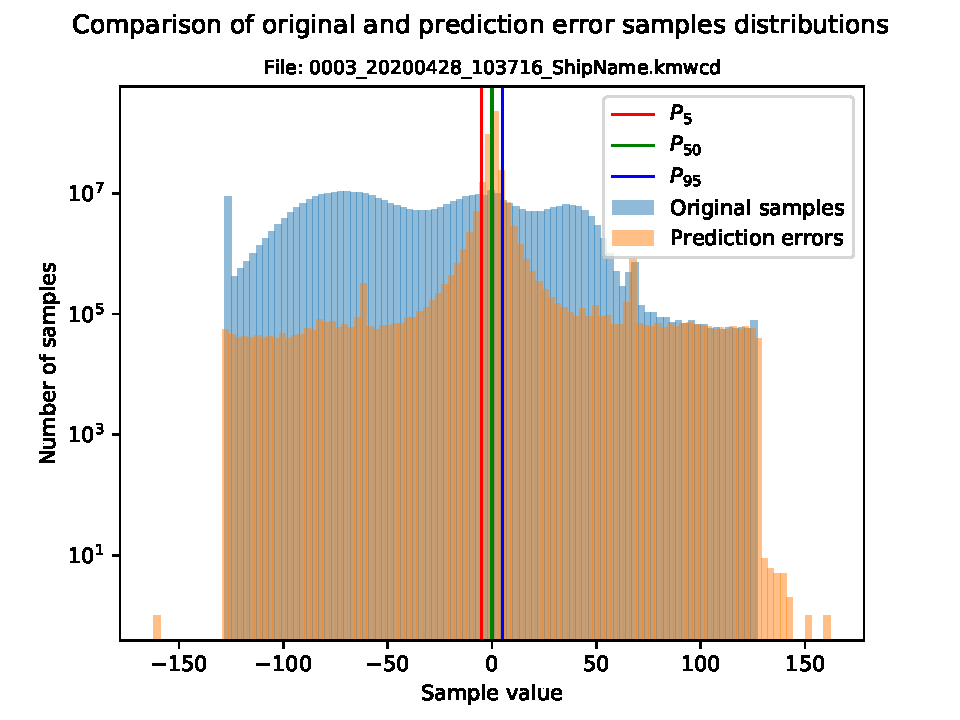
\includegraphics[width=\linewidth]{images/0003_20200428_103716_ShipName.kmwcd_hist.pdf}
		\caption{Histogram.}
		\label{fig:hist_003_kmall}
	\end{subfigure}%
	\begin{subfigure}{0.5\textwidth}
		\centering
		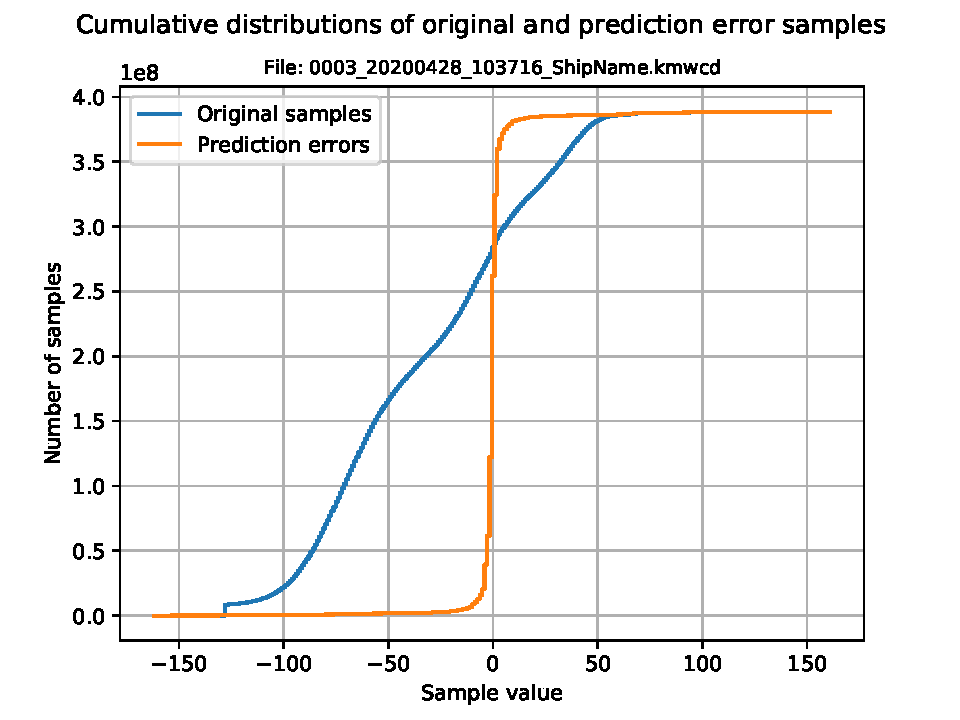
\includegraphics[width=\linewidth]{images/0003_20200428_103716_ShipName.kmwcd_hist_cum.pdf}
		\caption{Cumulative histogram.}
		\label{fig:cum_hist_003_kmall}
	\end{subfigure}
	\caption{Histograms showing the range reduction of MWC data from a EM 304.}
	\label{fig:0003_kmall}
\end{figure}

From the histograms we see that original data is distributed among the whole dynamic range, which would result in a poor compression ratio. After the preprocessing stage we propose, 90\% of the samples fall between -7 and +7.

If we look at the negentropies in Table \ref{tab:negentropies_kmall}. we see that for all the files the negentropy is higher after preprocessing. It is important to notice that we have estimated negentropies up to the 4th decimal, thus files with a very low negentropy are estimated with 0. We should also point out that the improvement for the last file is worse because it is the only one with phase information, which is almost incompressible (see Figure \ref{fig:wc_phase}).

\begin{table}[h!]
\normalsize
\centering
\begin{tabular}{|l|c|c|c|}
	\hline
	\rowcolor[HTML]{d6cefc} 
	\multicolumn{1}{|c|}{\cellcolor[HTML]{d6cefc}Filename}         & $J(X)$                           & $J(E)$                           & $J(E)/J(X)$ \\ \hline
	\cellcolor[HTML]{FFFFFF}0003\_20200428\_103716\_ShipName.kmwcd & \cellcolor[HTML]{FFFFFF}0.0004 & \cellcolor[HTML]{FFFFFF}0.0530 & 132.5     \\ \hline
	\cellcolor[HTML]{FFFFFF}0004\_20200428\_093723\_ShipName.kmwcd & \cellcolor[HTML]{FFFFFF}0.0000      & \cellcolor[HTML]{FFFFFF}0.0252 & -         \\ \hline
	\cellcolor[HTML]{FFFFFF}0039\_20200428\_115408\_ShipName.kmwcd & \cellcolor[HTML]{FFFFFF}0.0001 & \cellcolor[HTML]{FFFFFF}0.0146 & 146       \\ \hline
	0010\_20210409\_092708.kmwcd                                   & 0.0001                         & 0.0089                         & 89        \\ \hline
\end{tabular}
\caption{Negentropies of KMWCD files before and after preprocessing.}
\label{tab:negentropies_kmall}
\end{table}

We see that the KMALL stage has good results reducing the dynamic range of samples and increasing negentropy, but it would be almost useless if a general purpose compressor such as GZIP had a better compression ratio or was faster. For this reason, now we will compare the performance of \acrshort{fapec} with the KMALL stage and GZIP. We will proceed as in Wave and use the Euclidean distance metric proposed in section \ref{sec:euclidean}.

In Figure \ref{fig:kmall_compare} we plot the compression time and ratio for different files using \acrshort{fapec} and GZIP. We see that \acrshort{fapec} behaves much better than GZIP both in speed and ratio. For the particular case of a file with phase, both algorithms perform poorly in terms of ratio but \acrshort{fapec} is much faster. Besides, \acrshort{fapec} allows applying lossy compression to phase and lossless to amplitude.

\begin{figure}[h!]
	\begin{center}
		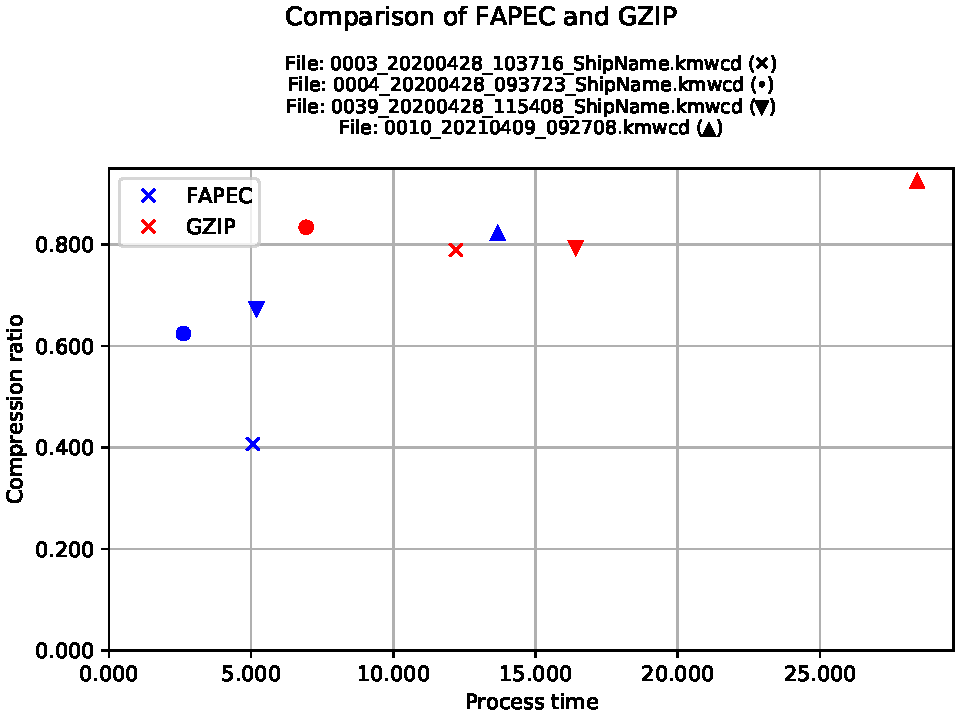
\includegraphics[scale=0.69]{images/2021-05-31T23:59:08.498586-results_kmall.csv_comparison.pdf}
	\end{center}
	\caption{Comparison of compressors showing that \acrshort{fapec} performs better both in time and ratio than GZIP.}
	\label{fig:kmall_compare}
\end{figure}

In Table \ref{tab:kmall_compare} we present the numerical values of the distances in Figure \ref{fig:kmall_compare}.

\begin{table}[h!]
\normalsize
\centering
\begin{tabular}{|l|c|c|}
	\hline
	\rowcolor[HTML]{d6cefc} 
	\multicolumn{1}{|c|}{\cellcolor[HTML]{d6cefc}Filename}         & FAPEC dist. & GZIP dist. \\ \hline
	\cellcolor[HTML]{FFFFFF}0003\_20200428\_103716\_ShipName.kmwcd & 5.0696      & 12.2123    \\ \hline
	\cellcolor[HTML]{FFFFFF}0004\_20200428\_093723\_ShipName.kmwcd & 2.6879      & 6.9850     \\ \hline
	\cellcolor[HTML]{FFFFFF}0039\_20200428\_115408\_ShipName.kmwcd & 5.2258      & 16.4260    \\ \hline
	0010\_20210409\_092708.kmwcd                                   & 13.6912     & 28.4271    \\ \hline
\end{tabular}
\caption{Euclidean distances for Figure \ref{fig:kmall_compare}.}
\label{tab:kmall_compare}
\end{table}

Our final considerations are that the stage has a McCabe complexity of 14, much smaller than 50 (see section \ref{sec:requirements}); and a memory occupation of 32 MB in the worst case. In conclusion, the proposed algorithm satisfies all requirements and specifications.